%!TEX root = ../rules-working.tex
%LTeX: enabled=false

\addedin{1B}{1B-figures}{

\begin{twocolumnfigure}

\begin{fitheight}{5.2\standardhexwidth}
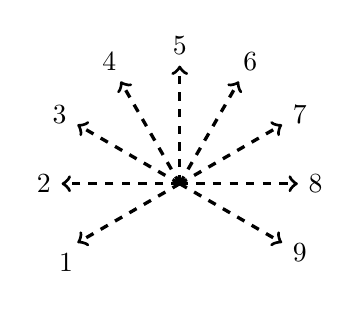
\begin{tikzpicture}
    \setfiguresize{-2.6}{-2.6}{+2.6}{+2.6}
    \begin{scope}
        \drawevenhexgrid{-2}{-2}{5}{5}
        \begin{scope}[dashed,very thick, ->]
            \draw (0,0) --   (90:1.5) node [anchor=270] {5};
            \draw (0,0) --   (60:1.5) node [anchor=240] {6};
            \draw (0,0) --   (30:1.5) node [anchor=210] {7};
            \draw (0,0) --    (0:1.5) node [anchor=180] {8};
            \draw (0,0) --  (330:1.5) node [anchor=150] {9};
            \draw (0,0) --  (210:1.5) node [anchor=60 ] {1};
            \draw (0,0) --  (180:1.5) node [anchor=0  ] {2};
            \draw (0,0) --  (150:1.5) node [anchor=330] {3};
            \draw (0,0) --  (120:1.5) node [anchor=300] {4};
        \end{scope}
        \drawaircraftcounter{0}{0}{90}{F-4}{}{}
     \end{scope}
\end{tikzpicture}
\end{fitheight}
\hfil
\begin{fitheight}{5.2\standardhexwidth}
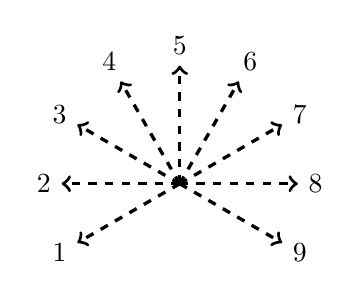
\begin{tikzpicture}
    \setfiguresize{-2.6}{-2.6}{+2.6}{+2.6}
    \begin{scope}[rotate=90]
        \drawevenhexgrid{-2}{-2}{5}{5}
        \begin{scope}[dashed,very thick,->]
            \draw (0,0) --   (0:1.5) node [anchor=270] {5};
            \draw (0,0) -- (330:1.5) node [anchor=240] {6};
            \draw (0,0) -- (300:1.5) node [anchor=210] {7};
            \draw (0,0) -- (270:1.5) node [anchor=180] {8};
            \draw (0,0) -- (240:1.5) node [anchor=150] {9};
            \draw (0,0) -- (120:1.5) node [anchor=30 ] {1};
            \draw (0,0) --  (90:1.5) node [anchor=0  ] {2};
            \draw (0,0) --  (60:1.5) node [anchor=330] {3};
            \draw (0,0) --  (30:1.5) node [anchor=300] {4};
        \end{scope}
        \drawaircraftcounter{0}{0}{0}{F-4}{}{}
    \end{scope}
\end{tikzpicture}
\end{fitheight}
\hfil
\begin{fitheight}{5.2\standardhexwidth}
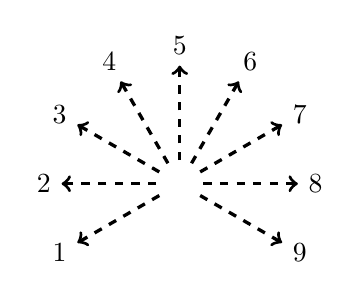
\begin{tikzpicture}
    \setfiguresize{-2.6}{-2.6}{+2.6}{+2.6}
    \begin{scope}[rotate=90]
        \drawevenhexgrid{-2}{-2}{5}{5}
        \begin{scope}[dashed,very thick,->]
            \draw   (0:0.3) --   (0:1.5) node [anchor=270] {5};
            \draw (330:0.3) -- (330:1.5) node [anchor=240] {6};
            \draw (300:0.3) -- (300:1.5) node [anchor=210] {7};
            \draw (270:0.3) -- (270:1.5) node [anchor=180] {8};
            \draw (240:0.3) -- (240:1.5) node [anchor=150] {9};
            \draw (120:0.3) -- (120:1.5) node [anchor=30 ] {1};
            \draw  (90:0.3) --  (90:1.5) node [anchor=0  ] {2};
            \draw  (60:0.3) --  (60:1.5) node [anchor=330] {3};
            \draw  (30:0.3) --  (30:1.5) node [anchor=300] {4};
        \end{scope}
        \drawaircraftcounter{-1}{0}{0}{F-4}{}{}
    \end{scope}
\end{tikzpicture}
\end{fitheight}

\figurecaption{figure:random-aaa}{Random Plotted AAA Fire}

\end{twocolumnfigure}
}
